% ECC26 talk -- toDMDc for Industrial Change Detection
% Session WeB9 "Fault Detection and Tolerance II", 15 min + 5 Q&A
% Build: latexmk -pdf slides.tex   (or: pdflatex slides.tex)
\documentclass[aspectratio=169,10pt]{beamer}

\usetheme{default}
\usecolortheme{seahorse}
\setbeamertemplate{navigation symbols}{}
\setbeamertemplate{footline}[frame number]

\usepackage{pifont}
\usepackage{graphicx}
\usepackage{amsmath,amssymb}
\usepackage{xcolor}
\usepackage{colortbl}
\usepackage{tikz}
\graphicspath{{figs/}}

% --- palette matches the figures -----------------------------------------
\definecolor{tblue}{HTML}{1F6FB2}
\definecolor{tred}{HTML}{D1495B}
\definecolor{tgreen}{HTML}{2A9D8F}
\definecolor{tgrey}{HTML}{6B7280}
\definecolor{tyellow}{HTML}{E0A800}
\setbeamercolor{structure}{fg=tblue}
\setbeamercolor{frametitle}{fg=tblue}
\setbeamerfont{frametitle}{series=\bfseries}

\newcommand{\yes}{\textcolor{tgreen}{\ding{51}}}
\newcommand{\no}{\textcolor{tred}{\ding{55}}}
\newcommand{\spine}[1]{%
  {\centering\Large\bfseries\color{tblue} #1\par}}

% --- capsule (stadium) for the 4-set Venn --------------------------------
\def\hh{1.55}% half-height = cap radius
\newcommand{\caps}[5]{% cx, cy, angle, halflen, color
  \begin{scope}[rotate around={#3:(#1,#2)}]
    \draw[fill=#5, fill opacity=0.30, draw=#5!75!black, line width=1pt, rounded corners=\hh cm]
      (#1-#4,#2-\hh) rectangle (#1+#4,#2+\hh);
  \end{scope}}
\tikzset{
  meth/.style={align=center, font=\scriptsize, fill=white, fill opacity=0.72,
               text opacity=1, rounded corners=2pt, inner sep=2.2pt},
  core/.style={align=center, font=\small\bfseries, fill=tblue!12, draw=tblue,
               line width=0.8pt, rounded corners=3pt, inner sep=3pt, text=tblue!85!black},
}

% --- title ----------------------------------------------------------------
\title[\bfseries toDMDc change detection]{Truncated Online DMD with Control\\for Industrial Change Detection}
\author[M. Wadinger]{\textbf{Marek Wadinger}\inst{1} \and Michal Kvasnica\inst{1} \and Yoshinobu Kawahara\inst{2}}
\institute[]{\inst{1} Slovak University of Technology in Bratislava \quad \inst{2} Osaka University \& RIKEN AIP}
\date{ECC 2026 \;\textbar\; WeB9 — Fault Detection and Tolerance II}

\begin{document}

% ===================== 1. COLD OPEN ======================================
\begin{frame}[plain]
  \titlepage
  \vspace{-1.2em}
  \begin{center}
    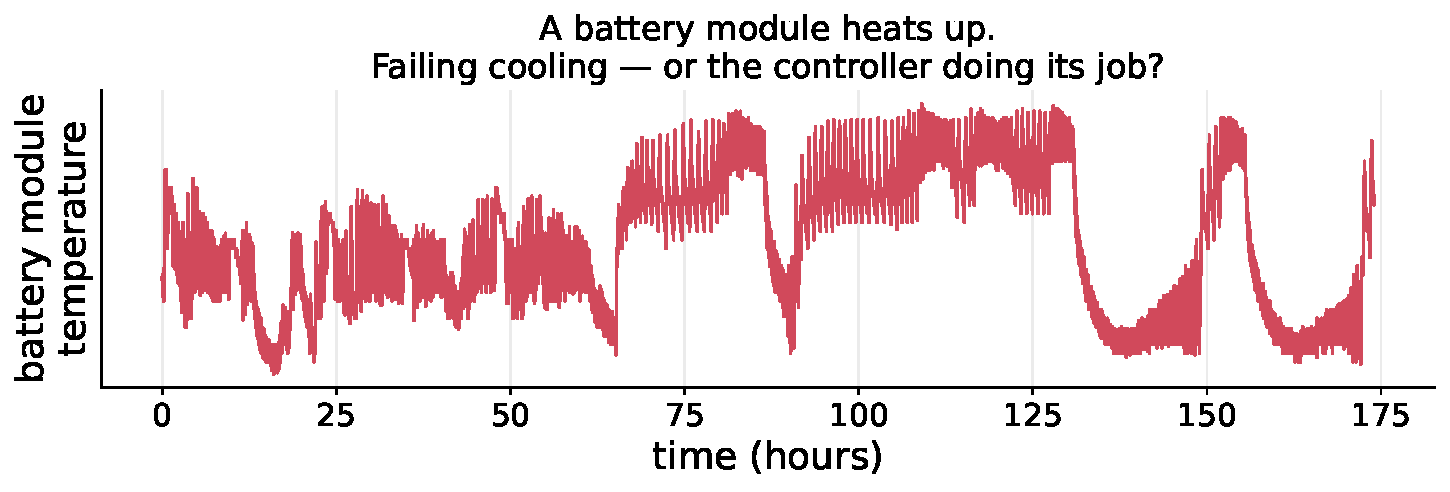
\includegraphics[width=0.78\linewidth]{fig_cold_open.pdf}
  \end{center}
\end{frame}

% Slide 1 speaker note lives in outline.md; cold open: stakes + spine, pause.

% ===================== 2. MONITORS DECAY =================================
\begin{frame}{We commission a monitor once. The plant runs for years.}
  % \begin{columns}[T]/newidth}
      \begin{itemize}
        \item Commissioned once $\rightarrow$ then the plant \textbf{ages, re-seasons, gets re-tuned}, gets new setpoints.
        \item The model is \textbf{frozen at day one}.
        \item The gap widens: \textcolor{tred}{false alarms climb, real faults hide}.
      \end{itemize}
      \vspace{0.6em}
      \begin{block}{The real requirement}
        Not a \emph{better} detector — one that \textbf{stays current} without a human re-tuning it.
      \end{block}
    % \end{column}
    % \begin{column}{0.44\linewidth}
    %   \centering
    %   \vspace{2em}
    %   {\itshape\color{tgrey}
    %   model fixed at $t_0$\\[0.4em]$\bullet$\\[0.4em] plant drifts away\\[0.4em]$\bullet$\\[0.4em] gap $=$ false alarms}
    % \end{column}
  % \end{columns}
\end{frame}

% ===================== 3. FOUR THINGS MOVE THE SIGNAL ====================
\begin{frame}{Four things move the signal — three are normal}
  \centering
  \resizebox{!}{0.74\textheight}{%
  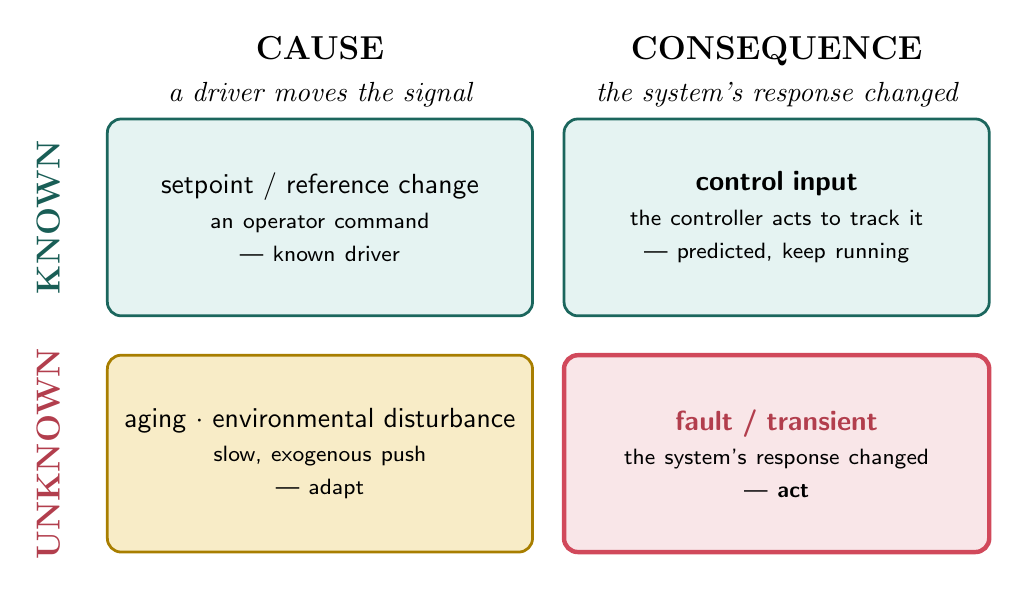
\begin{tikzpicture}[font=\sffamily,
    cell/.style={rounded corners=5pt, minimum width=5.4cm, minimum height=2.5cm,
                 align=center, line width=1pt, text width=5.0cm},
    colhdr/.style={font=\bfseries\large, align=center},
    rowhdr/.style={font=\bfseries\large, rotate=90, align=center}]

    % column headers
    \node[colhdr] at (0.0, 1.85) {CAUSE\\[1pt]{\normalsize\mdseries\itshape a driver moves the signal}};
    \node[colhdr] at (5.8, 1.85) {CONSEQUENCE\\[1pt]{\normalsize\mdseries\itshape the system's response changed}};
    % row headers
    \node[rowhdr, tgreen!60!black] at (-3.45, 0.0)  {KNOWN};
    \node[rowhdr, tred!85!black]   at (-3.45,-3.0)  {UNKNOWN};

    % --- cells -----------------------------------------------------------
    % Known x Cause  (normal)
    \node[cell, fill=tgreen!12, draw=tgreen!65!black] at (0.0,0.0)
      {setpoint / reference change\\[3pt]{\footnotesize an operator command\\ — known driver}};
    % Known x Consequence (normal -- the controller acting)
    \node[cell, fill=tgreen!12, draw=tgreen!65!black] at (5.8,0.0)
      {\textbf{control input}\\[3pt]{\footnotesize the controller acts to track it\\ — predicted, keep running}};
    % Unknown x Cause (normal-ish, adapt)
    \node[cell, fill=tyellow!22, draw=tyellow!75!black] at (0.0,-3.0)
      {aging $\cdot$ environmental disturbance\\[3pt]{\footnotesize slow, exogenous push\\ — adapt}};
    % Unknown x Consequence (FAULT)
    \node[cell, fill=tred!14, draw=tred, line width=1.6pt] at (5.8,-3.0)
      {\textbf{\textcolor{tred!85!black}{fault / transient}}\\[3pt]{\footnotesize the system's response changed\\ — \textbf{act}}};
  \end{tikzpicture}}

  \vspace{0.3em}
  {\footnotesize The controller acting (\textbf{known consequence}) is not a fault. An \textbf{unknown consequence} — the system changing — is.
  Same column, and a signal-watcher can't tell them apart: \textcolor{tred}{that is the gap.}}
\end{frame}

% ===================== 4. THE TRAP =======================================
\begin{frame}{The trap — and what we watch instead}
  \centering
  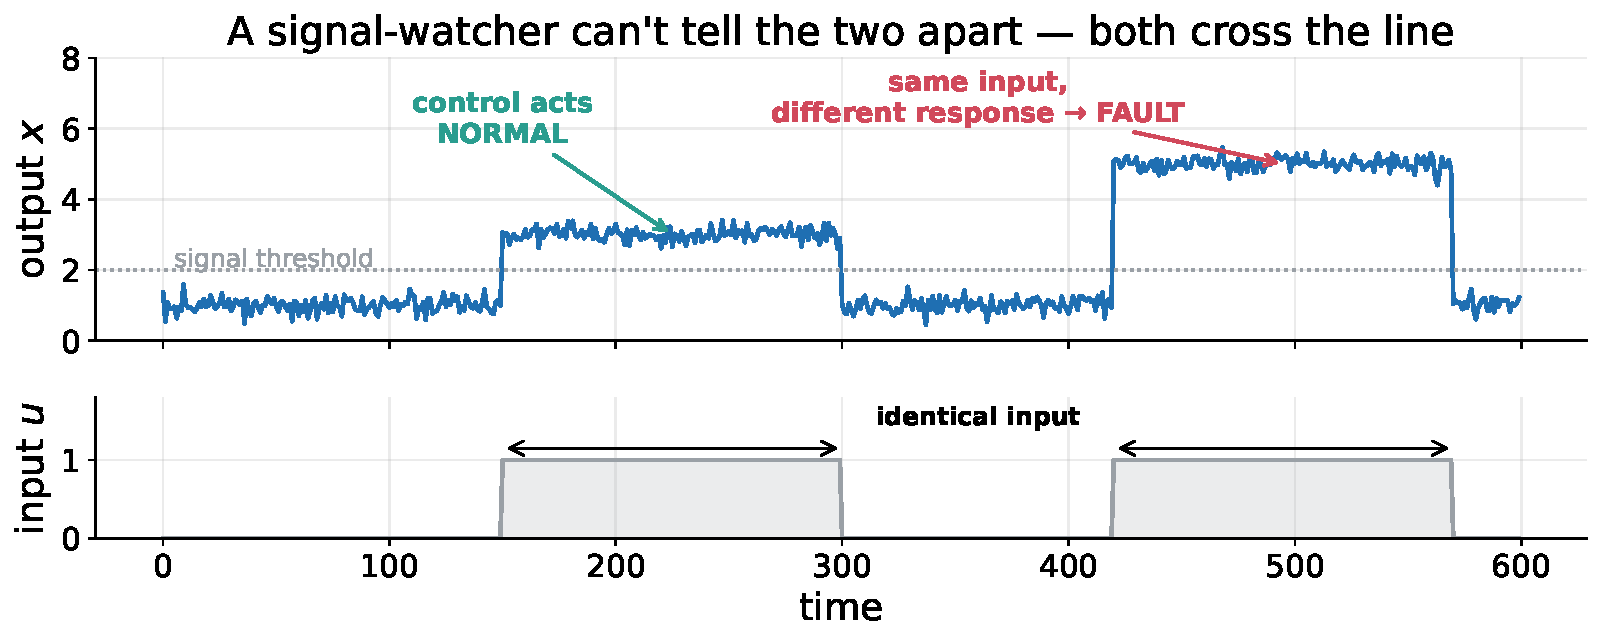
\includegraphics[width=0.9\linewidth]{fig_trap.pdf}\\
  \vspace{0.2em}
  {\footnotesize Two \emph{identical} inputs, two different responses. A signal-watcher (model free) alarms on both.}\\
  \textbf{We watch the \textcolor{tblue}{map} from input to state — only the second is a fault.}
\end{frame}

% ===================== 5. ONE MISSING BOX ================================
\begin{frame}{One missing box: only toDMDc fills all four}
  \centering
  \resizebox{!}{0.82\textheight}{%
  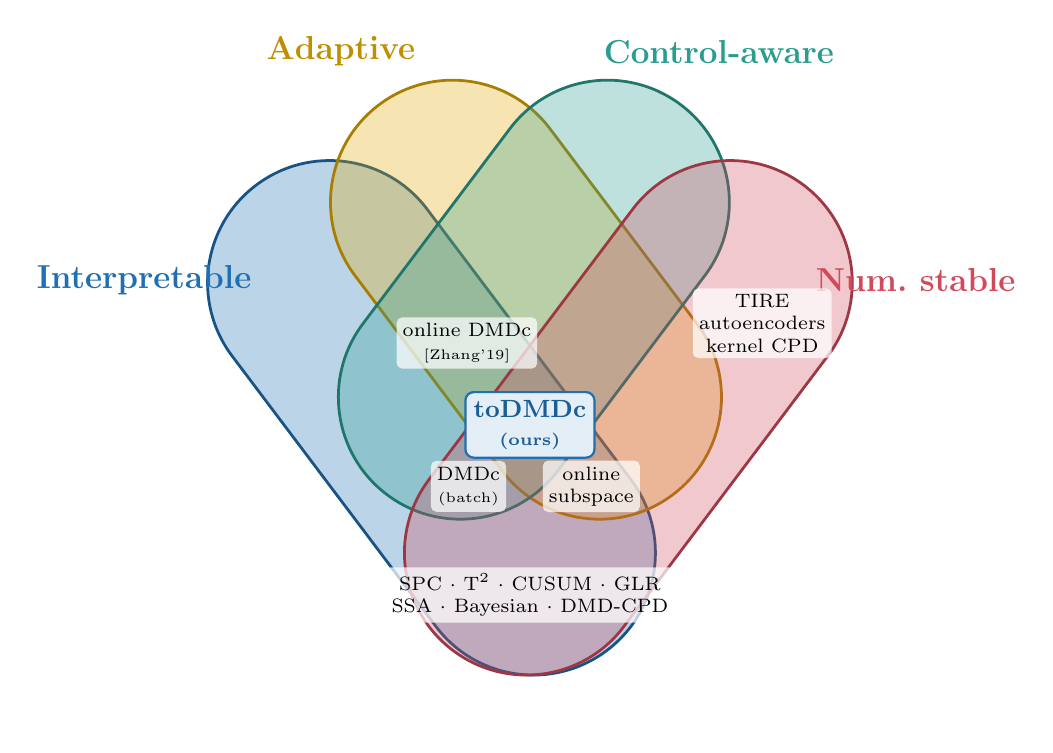
\begin{tikzpicture}[font=\sffamily]
    \caps{-1.25}{-0.05}{-53}{3.7}{tblue}    % A  Interpretable
    \caps{-0.05}{1.45}{-53}{3.1}{tyellow}   % B  Adaptive
    \caps{0.05}{1.45}{53}{3.1}{tgreen}      % C  Control-aware
    \caps{1.25}{-0.05}{53}{3.7}{tred}       % D  Num. stable

    % --- axis (set) names ------------------------------------------------
    \node[tblue,           font=\bfseries\large] at (-4.9, 1.7) {Interpretable};
    \node[tyellow!85!black,font=\bfseries\large] at (-2.4, 4.6) {Adaptive};
    \node[tgreen,          font=\bfseries\large] at ( 2.4, 4.6) {Control-aware};
    \node[tred,            font=\bfseries\large] at ( 4.9, 1.7) {Num.\ stable};

    % --- methods placed by what they offer (representative per region) ---
    \node[meth] at (-0.80, 0.90) {online DMDc\\{\tiny[Zhang'19]}};   % ABC  no stability
    \node[meth] at (-0.78,-0.92) {DMDc\\{\tiny(batch)}};             % ACD  no adaptivity
    \node[meth] at ( 0.78,-0.92) {online\\subspace};                % ABD  no control
    \node[meth] at ( 0.00,-2.30) {SPC $\cdot$ T$^2$ $\cdot$ CUSUM $\cdot$ GLR\\SSA $\cdot$ Bayesian $\cdot$ DMD-CPD}; % AD
    \node[meth] at ( 2.95, 1.15) {TIRE\\autoencoders\\kernel CPD}; % D-only black-box
    \node[core] at ( 0.00,-0.14) {toDMDc\\[-1pt]{\fontsize{6}{6}\selectfont(ours)}}; % ABCD
  \end{tikzpicture}}

  \vspace{-0.2em}
  {\footnotesize Representative methods per region; every prior family misses $\ge$1 box — \textbf{\textcolor{tblue}{toDMDc}} alone fills all four.}
\end{frame}

% ===================== 6. THE IDEA (CORE) ================================
\begin{frame}{The idea: watch the map, not the signal}
  \begin{columns}[T]
    \begin{column}{0.46\linewidth}
      \[ x_{k+1} = A\,x_k + B\,\textcolor{tblue}{\theta_k} \]
      The input $\theta_k$ is \emph{inside} the model $\Rightarrow$ a control-driven swing is \textbf{predicted} — it barely costs anything.
      \vspace{0.6em}
      \[ Q_k=\max\!\Big(0,\ \tfrac{E_{\text{test}}/c}{E_{\text{ref}}/a}-1\Big) \]
      same dynamics $\to Q\!\approx\!0$;\quad map moved $\to Q\!>\!0$.
    \end{column}
    \begin{column}{0.5\linewidth}
      \centering
      \footnotesize
      \begin{tabular}{ll}
        \textcolor{tgrey}{reference window $a$} & low error\\
        \textcolor{tblue}{test window $c$}      & error jumps on change\\
      \end{tabular}\\[1.2em]
      \begin{block}{}
        \centering We accounted for the input. What's left is the system.
      \end{block}
    \end{column}
  \end{columns}
  \vspace{0.6em}
  \spine{The controller acting is not a fault. The system changing is.}
\end{frame}

% ===================== 7. THE FIX (CONTRIBUTION) =========================
\begin{frame}{The fix: online truncation}
  \begin{columns}[T]
    \begin{column}{0.56\linewidth}
      \begin{itemize}
        \item Online DMDc fails on \textbf{small singular values} — inverting the noise floor makes the update blow up (literally divides by zero on rank-deficient data).
        \item We truncate to rank $r$ \textbf{online} — keep the directions that carry the dynamics, drop the noise floor — basis stays orthonormal.
        \item Cost drops to \textbf{$\mathcal{O}(mr^2)$ per step} — independent of history length.
      \end{itemize}
    \end{column}
    \begin{column}{0.42\linewidth}
      \centering
      \footnotesize\itshape
      \textcolor{tred}{no truncation}: update undefined\\
      $\downarrow$\\
      \textcolor{tblue}{rank-$r$ truncation}: bounded, real-time
    \end{column}
  \end{columns}
\end{frame}

% ===================== 8. GUARANTEES =====================================
\begin{frame}{Two guarantees you can stand behind}
  \begin{columns}[T]
    \begin{column}{0.5\linewidth}
      \begin{block}{Detection delay $\ge c$}
        The peak \emph{cannot} appear before the test window fills.\\
        \textcolor{tblue}{Window size = your reaction budget.}
      \end{block}
    \end{column}
    \begin{column}{0.5\linewidth}
      \begin{block}{Cost $\mathcal{O}(mr^2)$ / update}
        A handful of operations per sample, \textbf{independent of history length}.\\
        Runs inside the sample interval.
      \end{block}
    \end{column}
  \end{columns}
  \vspace{0.8em}
  \centering\footnotesize\itshape
  (Stationary-convergence and probabilistic bounds are in the paper — not claimed here as guarantees.)
\end{frame}

% ===================== 9. SPINE PROOF (two-tank) =========================
\begin{frame}{On a real nonlinear controlled plant}
  \centering
  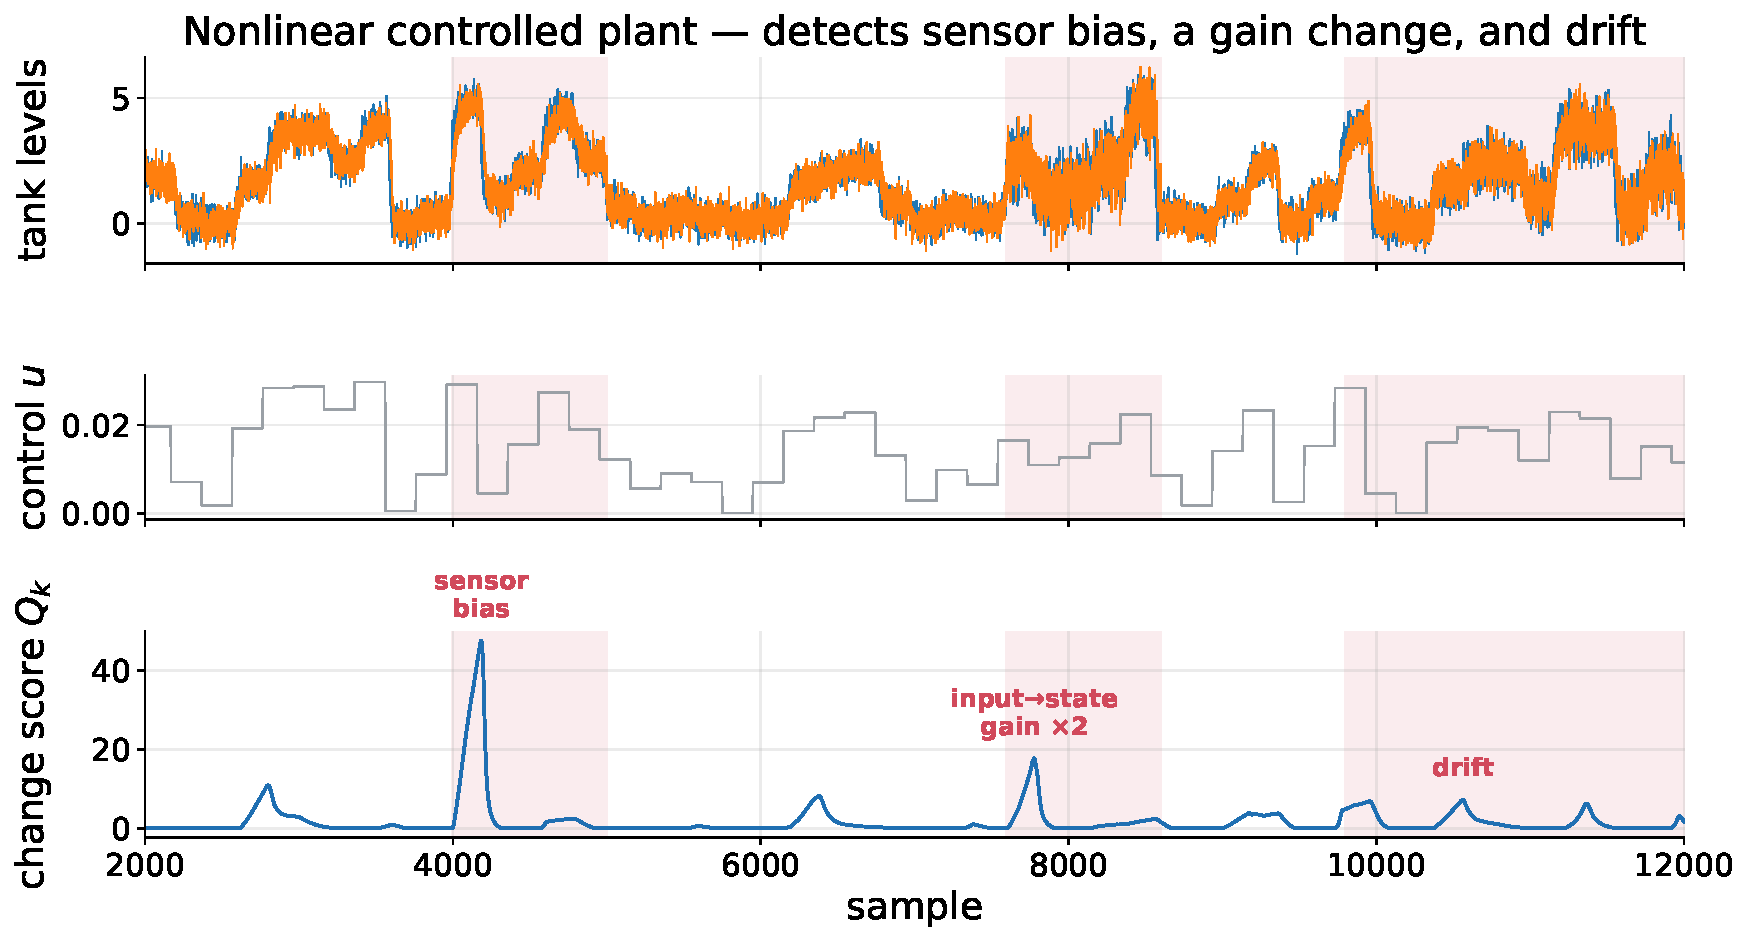
\includegraphics[width=0.88\linewidth]{fig_twotank_proof.pdf}\\
  \vspace{0.2em}
  {\footnotesize Two-tank with input delay. Detects all three injected faults — \textbf{sensor bias},
  an \textbf{input$\to$state gain change}, and \textbf{drift} — the gain change is exactly
  ``same input, different response''.}
\end{frame}

% ===================== 10. BESS HERO ====================================
\begin{frame}{Real-data win: catching it early}
  \centering
  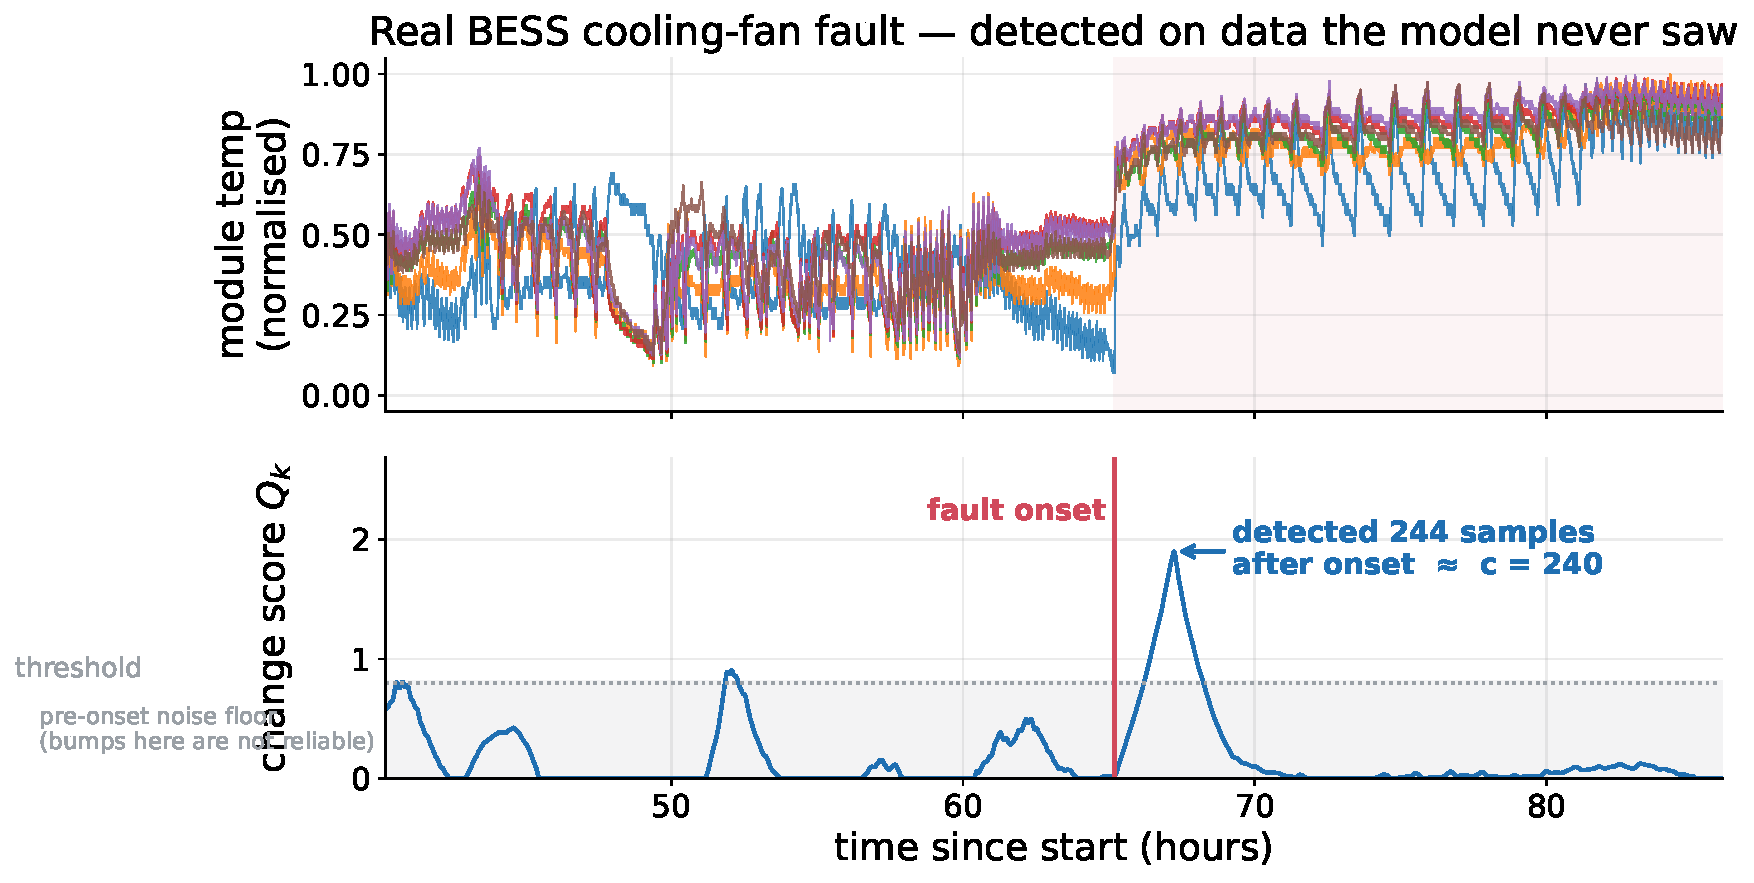
\includegraphics[width=0.9\linewidth]{fig_bess_hx10_crop.pdf}\\
  \vspace{0.2em}
  Real cooling-fan fault flagged with high confidence ($S_{\max}\!\approx\!2.0$) — and precursor
  peaks ($S\!\approx\!1.0$) lift \textbf{$\sim$2000 samples before the confirmed fault}, on data never seen.\\
  {\footnotesize (Suggestive of an unmodeled slow dynamic, not a confirmed mechanism — aligns with anomalies in earlier work.)}
\end{frame}

% ===================== 11. CLOSE ========================================
\begin{frame}{Closing the loop}
  \centering
  \renewcommand{\arraystretch}{1.3}
  \begin{itemize}
    \item Stays current on its own, tells the controller's actions apart from a real fault, delay you can size, cost you can afford.
    \item \textbf{Exactly the trigger a fault-tolerant scheme consumes} — detection ready to hand off to tolerance.
    \item Open source, one-line install, the BESS figures reproduce — \texttt{pip install reshift}.
  \end{itemize}
  \vspace{0.4em}
  \spine{The controller acting is not a fault. The system changing is.}
  \vspace{0.2em}
  \centering Thank you — happy to take questions.
\end{frame}

% ===================== BACKUP ===========================================
\appendix
\begin{frame}{Backup — two-tank, full run}
  \centering
  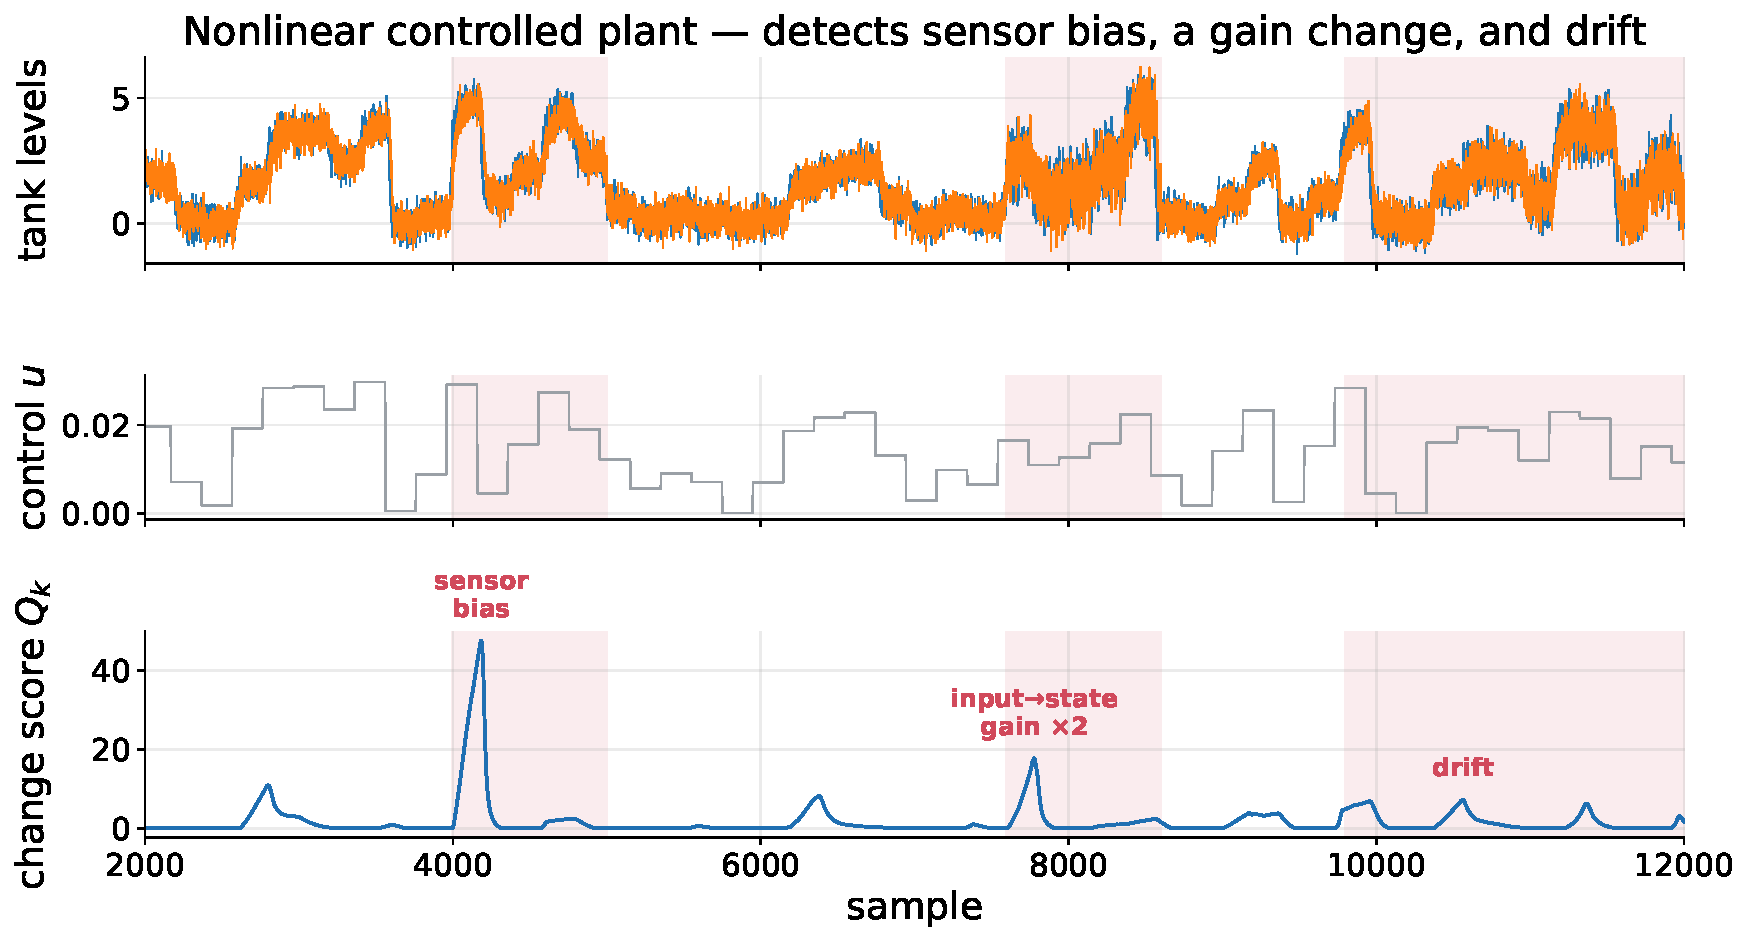
\includegraphics[width=0.86\linewidth]{fig_twotank_proof.pdf}\\
  All events: sensor bias, doubled response, linear drift. Score flat through control commands.
\end{frame}

\begin{frame}{Backup — BESS, full run (bidirectional)}
  \centering
  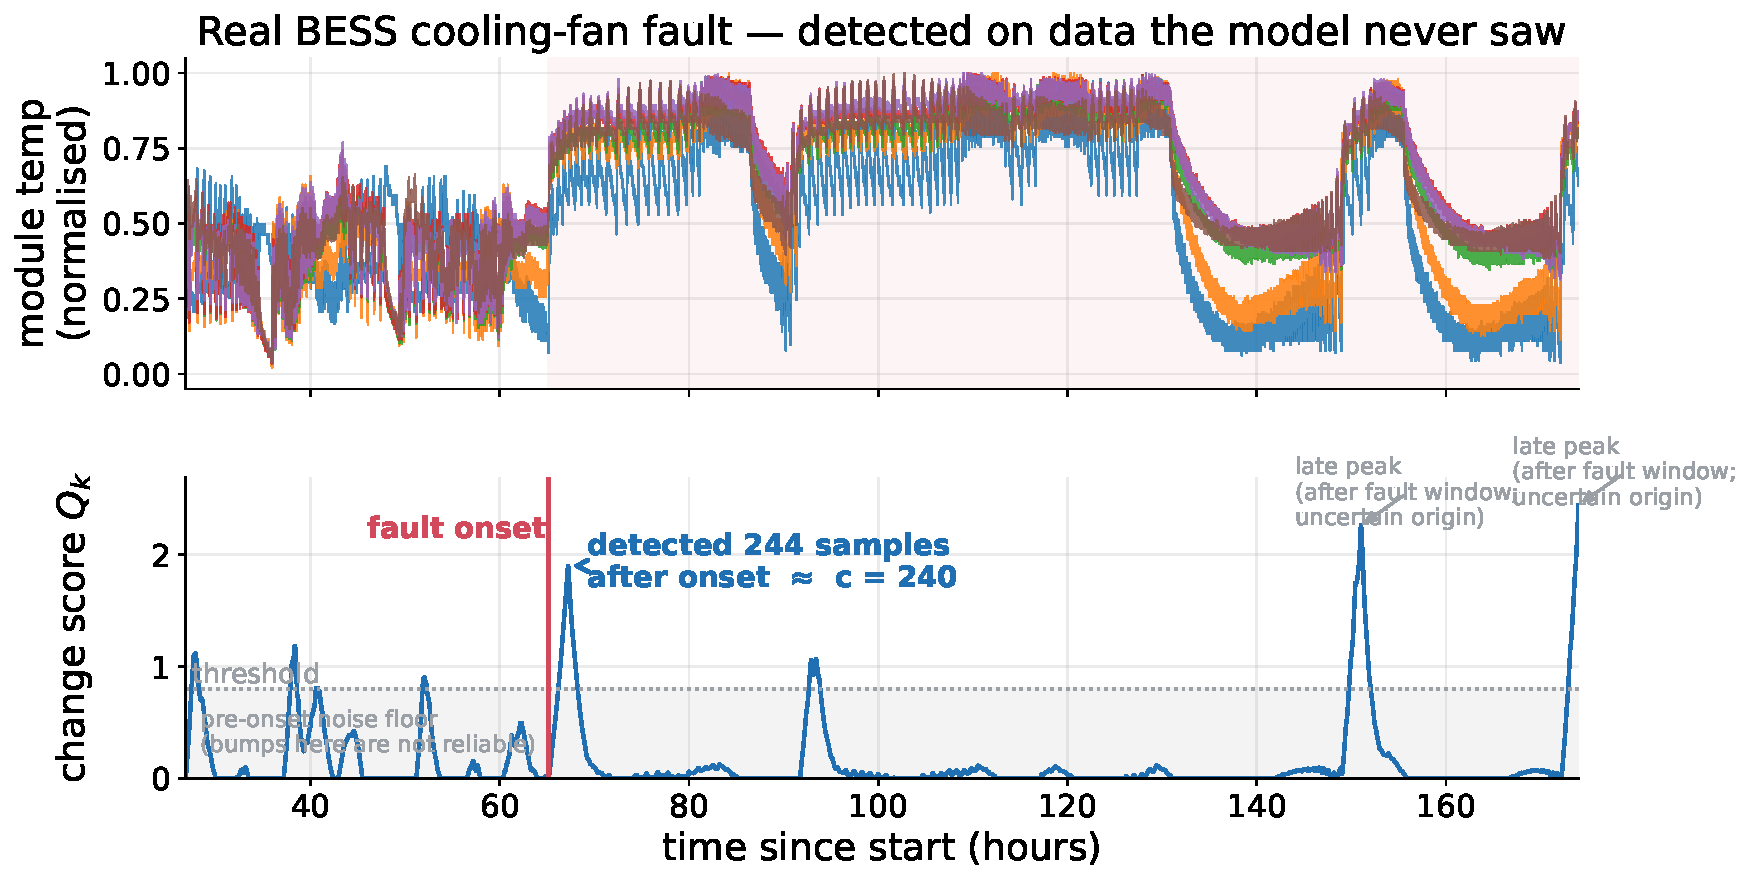
\includegraphics[width=0.86\linewidth]{fig_bess_hx10_full.pdf}\\
  Largest late peaks are return-to-normal transitions (bidirectional score).
\end{frame}

\begin{frame}{Backup — adaptation vs.\ detection (the hard question)}
  \small
  \textbf{Q:} \emph{A slow fault is a slow change — won't the learning window absorb it?}\\[0.4em]
  \textbf{A:} Detection precedes learning every step ($\ge c$ before any absorption).
  Faults are distinguished by \textbf{rate}, not magnitude — multi-resolution windows separate
  fault-rate from learning-rate. Honest limit: a change slower than $d$ is \emph{by design}
  treated as adaptation (= aging). Choosing $d$ sets that boundary.
\end{frame}

\end{document}
